\documentclass[11pt,a4paper]{article}

\usepackage{fullpage}
\usepackage{hyperref}
\usepackage{graphicx}
\usepackage{xcolor}
\definecolor{bg}{RGB}{39, 40, 34}

\usepackage{minted}
\usemintedstyle{monokai}
\setminted{
    bgcolor=bg,
    linenos,
    mathescape,
    autogobble,
    showspaces=false
}

\usepackage{fancyhdr}
\pagestyle{fancy}
\fancyhf{}

\renewcommand{\headrulewidth}{0pt}
\renewcommand{\footrulewidth}{0pt}

\fancypagestyle{firstpagefooter} {
	\lfoot{\tiny{Version: 06.10.2017}}
	\cfoot{}
	\rfoot{\thepage}

}

\lfoot{Name: Jakob Beckmann Legi: 17-945-866}
\rfoot{\thepage}

\begin{document}

\title{Advanced Systems Lab Report\\ \normalsize{Autumn Semester 2017}}
\author{Name: Jakob Beckmann\\Legi: 17-945-866}
\date{
	\vspace{4cm}
	\textbf{Grading} \\
	\vspace{0.5cm}
	\begin{tabular}{|c|c|}
		\hline  \textbf{Section} & \textbf{Points} \\
		\hline  1                &                 \\
		\hline  2                &                 \\
		\hline  3                &                 \\
		\hline  4                &                 \\
		\hline  5                &                 \\
		\hline  6                &                 \\
		\hline  7                &                 \\
		\hline \hline Total      &                 \\
		\hline
	\end{tabular}
}
\maketitle
\thispagestyle{firstpagefooter}

\newpage

\section{System Overview}
\subsection{Overall Design}
The overall design of the middleware created in this project is quite straight-forward. A single net-thread listens to a server socket and adds any requests sent to this socket to a blocking queue. A fixed number of worker threads then pull requests from the queue and process them one by one. Each of these worker threads is connected to all backend Memcached servers at all times. When a request is being processed by a worker thread, this thread calls to at least one Memcached server to handle the request. The only exception to this is an invalid request, such as an unknown command, in which case the middleware does not contact any backend servers.

\begin{figure}[h]
    \centering
    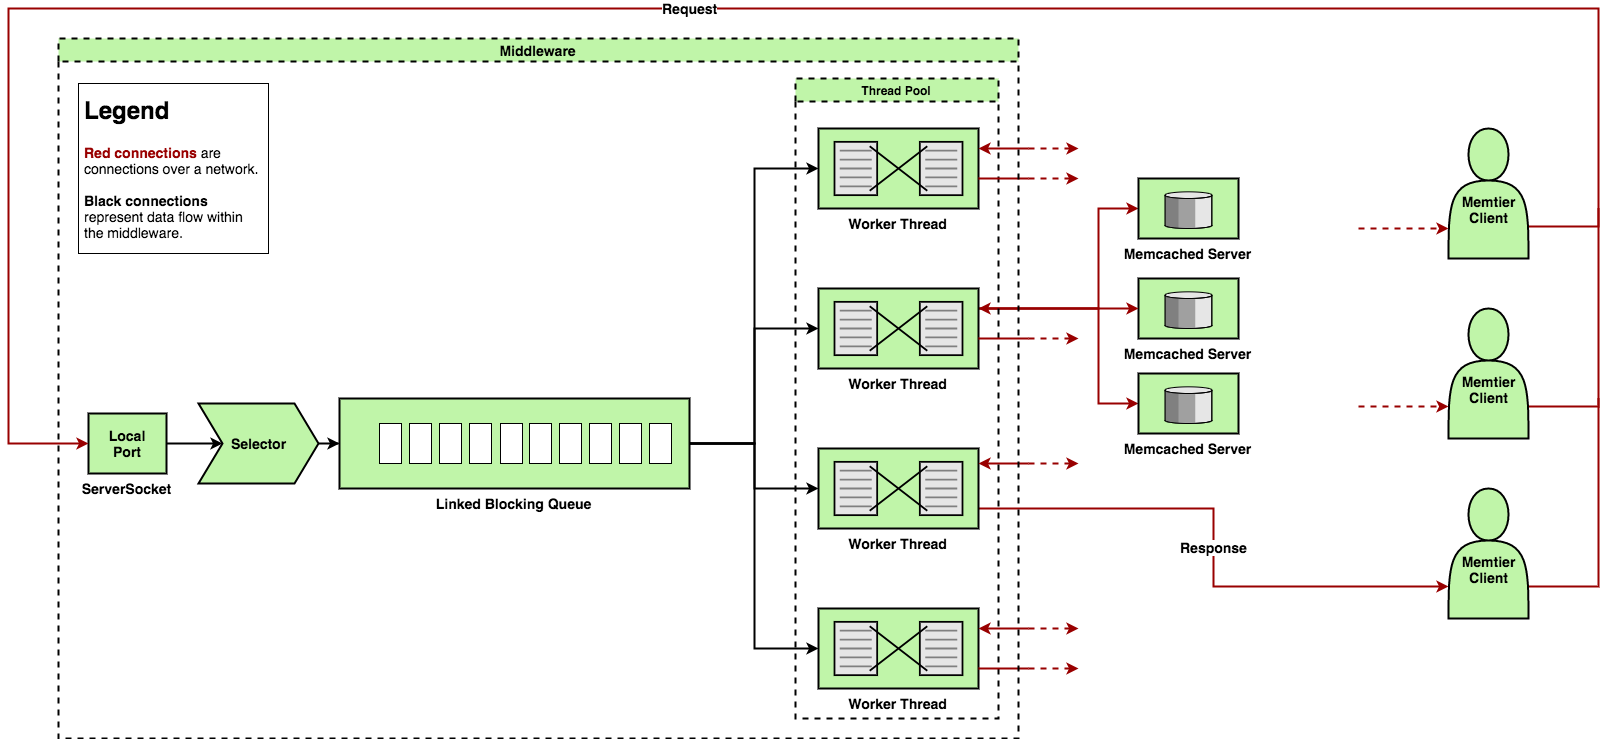
\includegraphics[width=\textwidth]{processing/graphics/system_overview.png}
    \caption{System Overview}
    \label{png::system_overview}
\end{figure}

As can be seen in figure \ref{png::system_overview}, a selector is attacked to the server socket in order to accept connections from clients. The key attached to the client connection is then passed with the request such that the workers can communicate the response back to the clients. The reason for the selector is to allow client connections to remain open until explicitly closed by the client. Hence the role of the selector is also to allow new connections and to add them to its internal register of client connections. Once in the internal register (the connection is accepted), the client can send a request which will be read by the net-thread and added to the queue with a reference to the client key. The worker threads then get requests off the queue and process them one by one. The workers first parse the request to get the command type. If the command is invalid, an error message is immediately sent back to the client associated with this request. Otherwise, the worker then communicates with the Memcached server(s) in order to store or retrieve data. The servers' response(s) are then parsed again to check for errors and statistics, and a response, potentially merged, is sent to the client.

\subsection{Selector}
The selector serves as a register for connected clients. It is used as passing a socket channel in the queue as part of the request forces the connection to be closed at completion of the request. Hence the selector accepts connections from clients and registers all connected clients. The selector then listens to the registered clients for messages sent to the server socket it is connected to and generates ``read events'' for each client sending messages to the socket. Simultaneously, the net-thread permanently checks for read events generated by the selector and reads data from the client associated with the event to a buffer. This buffer is then added as a request to the queue. Note that the selector key and a timestamp are added to the buffer to form a complete request on the queue. Moreover, note that the use of a selector forces to use non-blocking IO on the client side. However, this is not a problem since any read event guarantees that data can be read from the socket, hence avoiding the use of reading loops.

\subsection{Worker Threads}
A thread pool executor of fixed size is used to organise the worker threads. This has the advantage that it reduces thread environment switching if there is not need for an extra thread to be used. This could be the case when the connection to the Memcached servers are extremely fast. In such a case, the executor will not use more threads than than are available from the hardware as reusing the same thread to process the next request does not involve any overhead compared to switching to another thread to perform the same work. However, as soon as server service times increase, the thread pool allows to perform work on some thread while another is idle awaiting a response from Memcached. Moreover, the thread pool executor has the advantage that if some thread crashed during the execution of the middleware, it will automatically be relaunched. Hence it should in theory provide more stability to the system.

The worker threads perform close to the entirety of the work within the middleware. The reason these workers perform the most work is that the work can be performed concurrently and, ideally, it is performed in parallel. In the initial design, even the reading of the socket was performed by the workers to avoid creating a buffer (containing the message sent from the client) for each request. However, this lead to request duplication as the read event was active as long as nothing was read from the socket, hence repeatedly adding requests to the queue if the initial request had not already been read. This was easily caused by even non-significant queue times. Therefore the design was changed, at the cost of creating a byte buffer for each request.

When launching a thread, two buffers are created. One is used for temporary data while the other contains the response from Memcached to be sent back to clients. Note that all buffers used in the middleware are of size 16384 bytes as this allows for 10 keys of size 250 bytes and 10 values of 1024 (and some margin) to be stored in the buffer. The temporary data buffer is mostly used to interpret individual responses from the Memcached servers and its data is then added to the buffer containing the aggregate data for the client. Creating only two buffers for each worker has the goal to reduce dead times created by the garbage collector. Exactly how individual request types are handled by the middleware and how the buffers are utilised is explained in a later section.

Each worker is connected to all backend Memcached servers at all times. These channels are blocking to ensure that the worker awaits a response from the servers when reading from a channel. Should a worker crash, the thread pool executor will rebuild a thread to replace it and the connections to the servers should be reestablished. However, note that such a situation never occurred during testing.

\subsection{Requests}

\subsubsection{Sets}














Describe the implementation of your system and highlight design decisions relevant for the experiments. Explain how messages are parsed and how statistics are gathered in a multi-threaded setting. Provide figures containing all the threads and queues in your system (including the network and the memcached servers). Include illustrations that show how requests of different types are handled (e.g., components involved in processing the request and method calls). Please include all details necessary to understand artifacts and effects in your experiments that arise from your implementation choices.

\section{Baseline without Middleware (75 pts)}

In this experiments you study the performance characteristics of the memtier clients and memcached servers.

\subsection{One Server}

Both, for a read-only and write-only workload plot the throughput and the response time as a function of NumClients. All clients are connected to a single memcached instance.

Use 3 load generating VMs, with one memtier (CT=2) each, and vary the number of virtual clients (VC) per memtier thread between 1 and 32. Show how the behavior of the server changes as we add more clients.

\begin{center}
	\scriptsize{
		\begin{tabular}{|l|c|}
			\hline Number of servers                & 1                        \\
			\hline Number of client machines        & 3                        \\
			\hline Instances of memtier per machine & 1                        \\
			\hline Threads per memtier instance     & 2                        \\
			\hline Virtual clients per thread       & [1..32]                  \\
			\hline Workload                         & Write-only and Read-only \\
			\hline Multi-Get behavior               & N/A                      \\
			\hline Multi-Get size                   & N/A                      \\
			\hline Number of middlewares            & N/A                      \\
			\hline Worker threads per middleware    & N/A                      \\
			\hline Repetitions                      & 3 or more                \\
			\hline
		\end{tabular}
	}
\end{center}

\subsubsection{Explanation}

Describe in which phase the memcached servers are under-saturated, saturated, or over-saturated. Describe how throughput and response time correlate. Explain what further conclusions can be drawn from the experiment.


\subsection{Two Servers}

For a read-only and write-only workload plot throughput and response time as a function of NumClients. The clients are connected to two memcached instances.

Use 1 load generating VM, with one memtier (CT=1) connected to each memcached instance (two memcache instances in total), and vary the number of virtual clients (VC) per memtier thread between 1 and 32. Show how the behavior of the server changes and explain what conclusions we can draw from this experiment.

\begin{center}
	\scriptsize{
		\begin{tabular}{|l|c|}
			\hline Number of servers                & 2                        \\
			\hline Number of client machines        & 1                        \\
			\hline Instances of memtier per machine & 2                        \\
			\hline Threads per memtier instance     & 1                        \\
			\hline Virtual clients per thread       & [1..32]                  \\
			\hline Workload                         & Write-only and Read-only \\
			\hline Multi-Get behavior               & N/A                      \\
			\hline Multi-Get size                   & N/A                      \\
			\hline Number of middlewares            & N/A                      \\
			\hline Worker threads per middleware    & N/A                      \\
			\hline Repetitions                      & 3 or more (at least 1 minute each)                \\
			\hline
		\end{tabular}
	}
\end{center}

\subsubsection{Explanation}

Describe how this experiment compares to the previous section. Which results are the same and which ones differ? Explain what further conclusions can be drawn from the experiment.


\subsection{Summary}

Based on the experiments above, fill out the following table:

\begin{center}
	{Maximum throughput of different VMs.}
	\begin{tabular}{|l|p{2cm}|p{2cm}|p{4cm}|}
		\hline                        & Read-only workload & Write-only workload & Configuration gives max. throughput \\
		\hline One memcached server   &                    &                     &                                     \\
		\hline One load generating VM &                    &                     &                                     \\
		\hline
	\end{tabular}
\end{center}


Write at least two paragraphs about how both results relate. Describe what is the bottleneck of this setup is. If the maximum throughput for both experiments is the same, explain why. If it is not the case, explain why not. Write down key take-away messages about the behaviour of the memtier clients and the memcached servers.

\section{Baseline with Middleware (90 pts)}

In this set of experiments, you will have to use 1 load generator VM and 1 memcached server, measuring how the throughput of the system changes when increasing the number of clients. Scaling virtual clients inside memtier has to be done as explained in the previous sections. Plot both throughput and response time as measured on the middleware.

\subsection{One Middleware}

Connect one load generator machine (one instance of memtier with CT=2) to a single middleware and use 1 memcached server. Run a read-only and a write-only workload with increasing number of clients (between 2 and 64) and measure response time \emph{both at the client and at the middleware}, and plot the throughput and response time measured in the middleware.

Repeat this experiment for different number of worker threads inside the middleware: 8, 16, 32, 64.

\begin{center}
	\scriptsize{
		\begin{tabular}{|l|c|}
			\hline Number of servers                & 1                        \\
			\hline Number of client machines        & 1                        \\
			\hline Instances of memtier per machine & 1                        \\
			\hline Threads per memtier instance     & 2                        \\
			\hline Virtual clients per thread       & [1..32]                  \\
			\hline Workload                         & Write-only and Read-only \\
			\hline Multi-Get behavior               & N/A                      \\
			\hline Multi-Get size                   & N/A                      \\
			\hline Number of middlewares            & 1                        \\
			\hline Worker threads per middleware    & [8..64]                  \\
			\hline Repetitions                      & 3 or more (at least 1 minute each)                \\
			\hline
		\end{tabular}
	}
\end{center}

\subsubsection{Explanation}

Provide a detailed analysis of the results (e.g., bottleneck analysis, component utilizations, average queue lengths, system saturation). Add any additional figures and experiments that help you illustrate your point and support your claims.

\subsection{Two Middlewares}

Connect one load generator machine (two instances of memtier with CT=1) to two middlewares and use 1 memcached server. Run a read-only and a write-only workload with increasing number of clients (between 2 and 64) and measure response time \emph{both at the client and at the middleware}, and plot the throughput and response time as measured in the middleware.

Repeat this experiment for different number of worker threads inside the middleware: 8, 16, 32, 64.

If in your experiment the middleware is not the bottleneck, repeat the experiment that reaches the highest throughput but using two load generator VMs (each with 2x memtier CT=1) instead of one. Otherwise, explain how you know that the middlewares are the limiting factor in terms of throughput.

\begin{center}
	\scriptsize{
		\begin{tabular}{|l|c|}
			\hline Number of servers                & 1                        \\
			\hline Number of client machines        & 1                        \\
			\hline Instances of memtier per machine & 2                        \\
			\hline Threads per memtier instance     & 1                        \\
			\hline Virtual clients per thread       & [1..32]                  \\
			\hline Workload                         & Write-only and Read-only \\
			\hline Multi-Get behavior               & N/A                      \\
			\hline Multi-Get size                   & N/A                      \\
			\hline Number of middlewares            & 2                        \\
			\hline Worker threads per middleware    & [8..64]                  \\
			\hline Repetitions                      & 3 or more (at least 1 minute each)                \\
			\hline
		\end{tabular}
	}
\end{center}

\subsubsection{Explanation}

Provide a detailed analysis of the results (e.g., bottleneck analysis, component utilizations, average queue lengths, system saturation). Add any additional figures and experiments that help you illustrate your point and support your claims.

\subsection{Summary}

Based on the experiments above, fill out the following table. For both of them use the numbers from a single experiment to fill out all lines. Miss rate represents the percentage of GET requests that return no data. Time in the queue refers to the time spent in the queue between the net-thread and the worker threads.


\begin{center}
	{Maximum throughput for one middleware.}
	\begin{tabular}{|l|p{2cm}|p{2cm}|p{2cm}|p{2cm}|}
		\hline                                & Throughput & Response time & Average time in queue & Miss rate \\
		\hline Reads: Measured on middleware  &            &               &                       &           \\
		\hline Reads: Measured on clients     &            &               & n/a                   &           \\
		\hline Writes: Measured on middleware &            &               &                       & n/a       \\
		\hline Writes: Measured on clients    &            &               & n/a                   & n/a       \\
		\hline
	\end{tabular}
\end{center}

\begin{center}
	{Maximum throughput for two middlewares.}
	\begin{tabular}{|l|p{2cm}|p{2cm}|p{2cm}|p{2cm}|}
		\hline                                & Throughput & Response time & Average time in queue & Miss rate \\
		\hline Reads: Measured on middleware  &            &               &                       &           \\
		\hline Reads: Measured on clients     &            &               & n/a                   &           \\
		\hline Writes: Measured on middleware &            &               &                       & n/a       \\
		\hline Writes: Measured on clients    &            &               & n/a                   & n/a       \\
		\hline
	\end{tabular}
\end{center}

Based on the data provided in these tables, write at least two paragraphs summarizing your findings about the performance of the middleware in the baseline experiments.

\section{Throughput for Writes (90 pts)}

\subsection{Full System}

Connect three load generating VMs to two middlewares and three memchached servers. Run a write-only experiment.
You need to plot throughput and response time measured on the middleware as a function of number of clients. The measurements have to be performed for 8, 16, 32 and 64 worker threads inside each middleware.

\begin{center}
	\scriptsize{
		\begin{tabular}{|l|c|}
			\hline Number of servers                & 3          \\
			\hline Number of client machines        & 3          \\
			\hline Instances of memtier per machine & 2          \\
			\hline Threads per memtier instance     & 1          \\
			\hline Virtual clients per thread       & [1..32]    \\
			\hline Workload                         & Write-only \\
			\hline Multi-Get behavior               & N/A        \\
			\hline Multi-Get size                   & N/A        \\
			\hline Number of middlewares            & 2          \\
			\hline Worker threads per middleware    & [8..64]    \\
			\hline Repetitions                      & 3 or more (at least 1 minute each)  \\
			\hline
		\end{tabular}
	}
\end{center}

\subsubsection{Explanation}

Provide a detailed analysis of the results (e.g., bottleneck analysis, component utilizations, average queue lengths, system saturation). Add any additional figures and experiments that help you illustrate your point and support your claims.

\subsection{Summary}

Based on the experiments above, fill out the following table with the data corresponding to the maximum throughput point for all four worker-thread scenarios.

\begin{center}
	{Maximum throughput for the full system}
	\begin{tabular}{|l|p{1.5cm}|p{1.5cm}|p{1.5cm}|p{1.5cm}|}
		\hline                                            & WT=8 & WT=16 & WT=32 & WT=64 \\
		\hline Throughput (Middleware)                    &      &       &       &       \\
		\hline Throughput (Derived from MW response time) &      &       &       &       \\
		\hline Throughput (Client)                        &      &       &       &       \\
		\hline Average time in queue                      &      &       &       &       \\
		\hline Average length of queue                    &      &       &       &       \\
		\hline Average time waiting for memcached         &      &       &       &       \\
		\hline
	\end{tabular}
\end{center}

Based on the data provided in these tables, draw conclusions on the state of your system for a variable number of worker threads.

\section{Gets and Multi-gets (90 pts)}

For this set of experiments you will use three load generating machines, two middlewares and three memcached servers. Each memtier instance should have 2 virtual clients in total and the number of middleware worker threads is 64, or the one that provides the highest throughput in your system (whichever number of threads is smaller).

For multi-GET workloads, memtier will generate a mixture of SETs, GETs, and multi-GETs. Memtier only allows to specify the maximum number of keys in a multi-GET request. Therefore, be aware that requests can also contain fewer keys than the provided value. It is recommended to record the average size of the multi-GETs. You will have to measure response time on the client as a function of multi-get size, with and without sharding on the middlewares.

\subsection{Sharded Case}

Run multi-gets with 1, 3, 6 and 9 keys (memtier configuration) with sharding enabled (multi-gets are broken up into smaller multi-gets and spread across servers). Plot average response time as measured on the client, as well as the 25th, 50th, 75th, 90th and 99th percentiles.

\begin{center}
	\scriptsize{
		\begin{tabular}{|l|c|}
			\hline Number of servers                & 3                       \\
			\hline Number of client machines        & 3                       \\
			\hline Instances of memtier per machine & 2                       \\
			\hline Threads per memtier instance     & 1                       \\
			\hline Virtual clients per thread       & 2     		            \\
			\hline Workload                         & memtier-default             \\
			\hline Multi-Get behavior               & Sharded                 \\
			\hline Multi-Get size                   & [1..9]                  \\
			\hline Number of middlewares            & 2                       \\
			\hline Worker threads per middleware    & max. throughput config. \\
			\hline Repetitions                      & 3 or more (at least 1 minute each)               \\
			\hline
		\end{tabular}
	}
\end{center}

\subsubsection{Explanation}

Provide a detailed analysis of the results (e.g., bottleneck analysis, component utilizations, average queue lengths, system saturation). Add any additional figures and experiments that help you illustrate your point and support your claims.

\subsection{Non-sharded Case}

Run multi-gets with 1, 3, 6 and 9 keys (memtier configuration) with sharding disabled. Plot average response time as measured on the client, as well as the 25th, 50th, 75th, 90th and 99th percentiles.

\begin{center}
	\scriptsize{
		\begin{tabular}{|l|c|}
			\hline Number of servers                & 3                       \\
			\hline Number of client machines        & 3                       \\
			\hline Instances of memtier per machine & 2                       \\
			\hline Threads per memtier instance     & 1                       \\
			\hline Virtual clients per thread       & 2                		 \\
			\hline Workload                         & memtier-default             \\
			\hline Multi-Get behavior               & Non-Sharded             \\
			\hline Multi-Get size                   & [1..9]                  \\
			\hline Number of middlewares            & 2                       \\
			\hline Worker threads per middleware    & max. throughput config. \\
			\hline Repetitions                      & 3 or more (at least 1 minute each)               \\
			\hline
		\end{tabular}
	}
\end{center}

\subsubsection{Explanation}

Provide a detailed analysis of the results (e.g., bottleneck analysis, component utilizations, average queue lengths, system saturation). Add any additional figures and experiments that help you illustrate your point and support your claims.

\subsection{Histogram}

For the case with 6 keys inside the multi-get, display four histograms representing the sharded and non-sharded response time distribution, both as measured on the client, and inside the middleware. Choose the bucket size in the same way for all four, and such that there are at least 10 buckets on each of the graphs.

\subsection{Summary}

Provide a detailed comparison of the sharded and non-shareded modes. For which multi-GET size is sharding the preferred option? Provide a detailed analysis of your system. Add any additional figures and experiments that help you illustrate your point and support your claims.

\section{2K Analysis (90 pts)}

For 3 client machines (with 64 total virtual clients per client VM) measure the throughput and response time of your system in a 2k experiment with repetitions. All GET operations have a single key. Investigate the following parameters:

\begin{itemize}

	\item Memcached servers: 2 and 3
	\item Middlewares: 1 and 2
	\item Worker threads per MW: 8 and 32

\end{itemize}

Repeat the experiment for (a)~a write-only, (b)~a read-only, and (c)~a 50-50-read-write workload.
For each of the three workloads, what is the impact of these parameters on throughput, respectively response time?

\begin{center}
	\scriptsize{
		\begin{tabular}{|l|c|}
			\hline Number of servers                & 2 and 3                                     \\
			\hline Number of client machines        & 3                                           \\
			\hline Instances of memtier per machine & 2                                           \\
			\hline Threads per memtier instance     & 1                                           \\
			\hline Virtual clients per thread       & 32                                     \\
			\hline Workload                         & Write-only, Read-only, and 50-50-read-write \\
			\hline Multi-Get behavior               & N/A                                         \\
			\hline Multi-Get size                   & N/A                                         \\
			\hline Number of middlewares            & 1 and 2                                     \\
			\hline Worker threads per middleware    & 8 and 32                                    \\
			\hline Repetitions                      & 3 or more (at least 1 minute each)                                   \\
			\hline
		\end{tabular}
	}
\end{center}

\section{Queuing Model (90 pts)}

Note that for queuing models it is enough to use the experimental results from the previous sections. It is, however, possible that the numbers you need are not only the ones in the figures we asked for, but also the internal measurements that you have obtained through instrumentation of your middleware.

\subsection{M/M/1}

Build queuing model based on Section 4 (write-only throughput) for each worker-thread configuration of the middleware. Use one M/M/1 queue to model your entire system. Motivate your choice of input parameters to the model. Explain for which experiments the predictions of the model match and for which they do not.

\subsection{M/M/m}

Build an M/M/m model based on Section 4, where each middleware worker thread is represented as one service.  Motivate your choice of input parameters to the model. Explain for which experiments the predictions of the model match and for which they do not.

\subsection{Network of Queues}

Based on Section 2, build a network of queues which simulates your system. Motivate the design of your network of queues and relate it wherever possible to a component of your system. Motivate your choice of input parameters for the different queues inside the network. Perform a detailed analysis of the utilization of each component and clearly state what the bottleneck of your system is. Explain for which experiments the predictions of the model match and for which they do not.

\end{document}
